%!TEX root = ../thesis.tex

\chapter{The Experiment \Eonefourthree}\label{chap:results}
%\iffalse 
\lettrine{I}{n} this chapter, the results from experiment \textsc{E143} \cite{kortenE143} are presented. Firstly, the beam time experience is detailed in \cref{sec:chap3:beamtimestory}. Following this introduction, the chapter presents the results. It covers the identification process (\cref{sec:chap3:identification}), the analysis of isochronicity curves (\cref{sec:chap3:isochronicity}), and their implications for mass resolving power (\cref{sec:chap3:massresolvingpower}), demonstrating the highest resolving power ever achieved in \textsc{IMS} and ranking among the highest at storage rings. The subsequent section, \cref{sec:chap3:massmeasurements}, highlights some of the most precise mass measurements achieved in storage rings, highlighting the improvement on the mass uncertainty of \,\isotope{69}{As} and a $3\sigma$ mass deviation on \,\isotope{72}{As}, in agreement with a recent study. Finally, the chapter presents the half-life measurements, including the first measurement of the nuclear two-photon decay half-life in \,\isotope{72}{Ge} (\cref{subsec:chap3:hl-twophoton}) and measurements of pure single-photon decays (\cref{subsec:chap3:purephoton}).
%HERE ASSSSSSSSSSSSSSSSSSSSSSSSS

%Only the 245 MHz data was connected to the NTCAP as previously discussed, therefore only we have a broad band measurement for this detector. Consequently, from now on until the half-life measurement of the nuclear two-photon decay half-life \cref{subsec:chap3:hl-twophoton} we are always presenting results from the 245 Schottky.
%\iffalse
\section{Beam time story}\label{sec:chap3:beamtimestory}
%Add about the proposals?
\begin{figure}[h] % 'p' places the figure on a page containing only floats
  \centering
  \subfloat[First part of the beam time schedule of the experiment \textsc{E143}.]{
      \includegraphics[width=0.46\textwidth]{beamtimeE1431.png}
      \label{fig:chap3:beamtime_schedule_1}
  }
  \hspace{0.5cm}
  \subfloat[Second part of the beam time schedule of the experiment \textsc{E143}.]{
      \includegraphics[width=0.46\textwidth]{beamtimeE1432.png}
      \label{fig:chap3:beamtime_schedule_2}
  }
  \caption{Beam time schedule for experiment \textsc{E143} conducted in May and June/July $2021$.}
  \label{fig:chap3:beamtime_schedule}
\end{figure}
\Cref{fig:chap3:beamtime_schedule} shows a schematic overview of the beam time schedules that took place in May $2021$ (\cref{fig:chap3:beamtime_schedule_1}) and between June-July $2021$ (\cref{fig:chap3:beamtime_schedule_2}). In both, the experimental set-up is depicted in orange. It encompasses (among others) various stages including energy calibration post-stripper, determination of the \gt ion-optical parameter with the electron cooler and set-up of the data acquisition system. In blue are highlighted the low-resolution settings where we had broader peak widths, hindering the resolution of low-lying states. In green are outlined the high-resolution settings from where we can find the data of the results for \germanium and for \,\isotope{70}{Se} obtained within this thesis.
\newpar
The transitions from low-resolution to high-resolution settings were achieved by changing the energy of the ions and by trying different scraper positions. By changing the energy we can move the isochronous condition to other mass-to-charge ratio while by searching for different scrapper positions we can reduce the momentum spread.
\newpar
As we can see in \cref{fig:chap3:beamtime_schedule_1} and in \cref{fig:chap3:beamtime_schedule_2}, most of the beam time was spent into the set-up (taking also into account the low-resolution settings). This was due to the novelties of the methodology:
\begin{itemize}
  \item First time observed overlapping harmonics in \textsc{IMS}.
  \item Shortest half-live measured with \textsc{S+IMS}.
  \item First time achieving such high resolution in \textsc{IMS}.
\end{itemize}


During the first beam time (see \cref{fig:chap3:beamtime_schedule_1}), after achieving a high-resolution setting for \,\ion{72}{Ge}{32} it was decided to shift the focus on searching of a new low-lying $0^+$ state in \,\ion{70}{Se}{34}. This was the second motivation of the experiment proposal \cite{kortenE143}. As an intermediate step, we tried to calibrate the setting on \,\ion{52}{Mn}{25} in order to try to resolve its $377.749 (5)$\,keV~\cite{ENSDF} isomeric state. However, the setting was not on \,\ion{52}{Mn}{25}, it was misidentified. Nevertheless, the mass resolving power was good enough and the focus was shifted to \,\ion{70}{Se}{34}. For that, while having $\gamma_t$ fixed, the energy of the ions was changed systematically since we did not have the necessary analysis tool to determine the exact energy inside the ring. At the end a high-resolution setting was achieved, but not isochronous for the targeted ion, as can be seen in the results \cref{fig:chap3:iso70SeMay}. 
After several hours of measurement on \,\ion{70}{Se}{34}, there was no direct evidence of an isomer detected. Consequently, it was decided to shift back to the \,\ion{72}{Ge}{32} setting, where we could recover a very similar high-resolution setting as previously, albeit with extended operation time (approximately $8$\,hours) to increase the statistics. 

Due to the challenges faced during the \textbf{first} implementation of \textsc{S+IMS} (see \cref{chap:chap2:methodology}) at the \textsc{ESR}, and because the full requested beam time was not allocated \cite{kortenE143}, the second part of the proposal did not record enough events. 
Recognizing the difficulties and the high discovery potential by the \textsc{GSI} management, a follow-up beam time was conducted in June-July $2021$ focusing on \,\ion{70}{Se}{34}.
In this case, initially the set-up was aligned to \,\ion{72}{Ge}{32} to compare with the setting used in the May run. However, the mass resolving power achieved was not even enough to resolve nuclides within $4$\,MeV. Nonetheless, we still could compare the main features such as the center frequency. This led us to use a higher harmonic ($h$) since the revolution frequencies were smaller than in the May beam time.
Consequently, the focus was switched to \,\ion{70}{Se}{34}. In that mass-to-charge region both \,\ion{72}{Br}{35} and its $100$~keV isomer were present. The objective was to reach a setting where this isomer could be distinctly resolved in addition to be expectant to find a peak around \,\ion{70}{Se}{34}, indicating a \textbf{new} low-lying $0^+$ state. 
%\fi 
\section{Ion identification}\label{sec:chap3:identification}
One of the key characteristics of Schottky-induced signals in storage rings is their intrinsic periodicity. 
This periodicity allows for the identification of each observed peak. Our detectors do not work in the frequency range where the revolution frequency of the ions (\textsc{eigenfrequency}) is observed, but rather they work at a higher frequency where multiples of it, denoted by $h$, are observed (refer to \cref{subsec:chap2:detection} for more information).
Due to this, in the broadband measurements, we encounter harmonic overlap, a phenomenon detailed in \cref{apdx:harmonicoverlap} and \cref{subsubsec:chap2:harmonicoverlapping}. Consequently, the periodicity observed in our data does not imply that all peaks correspond to unique ions; some are repeated, like the ones shown in \cref{fig:chap3:ident1D}. This repetition is leveraged to unambiguously identify each peak.
\begin{figure}[hbt] % 'p' places the figure on a page containing only floats
  \centering
  \subfloat[Most expected fragments for the \germanium setting from \textsc{LISE++} calculations.]{
      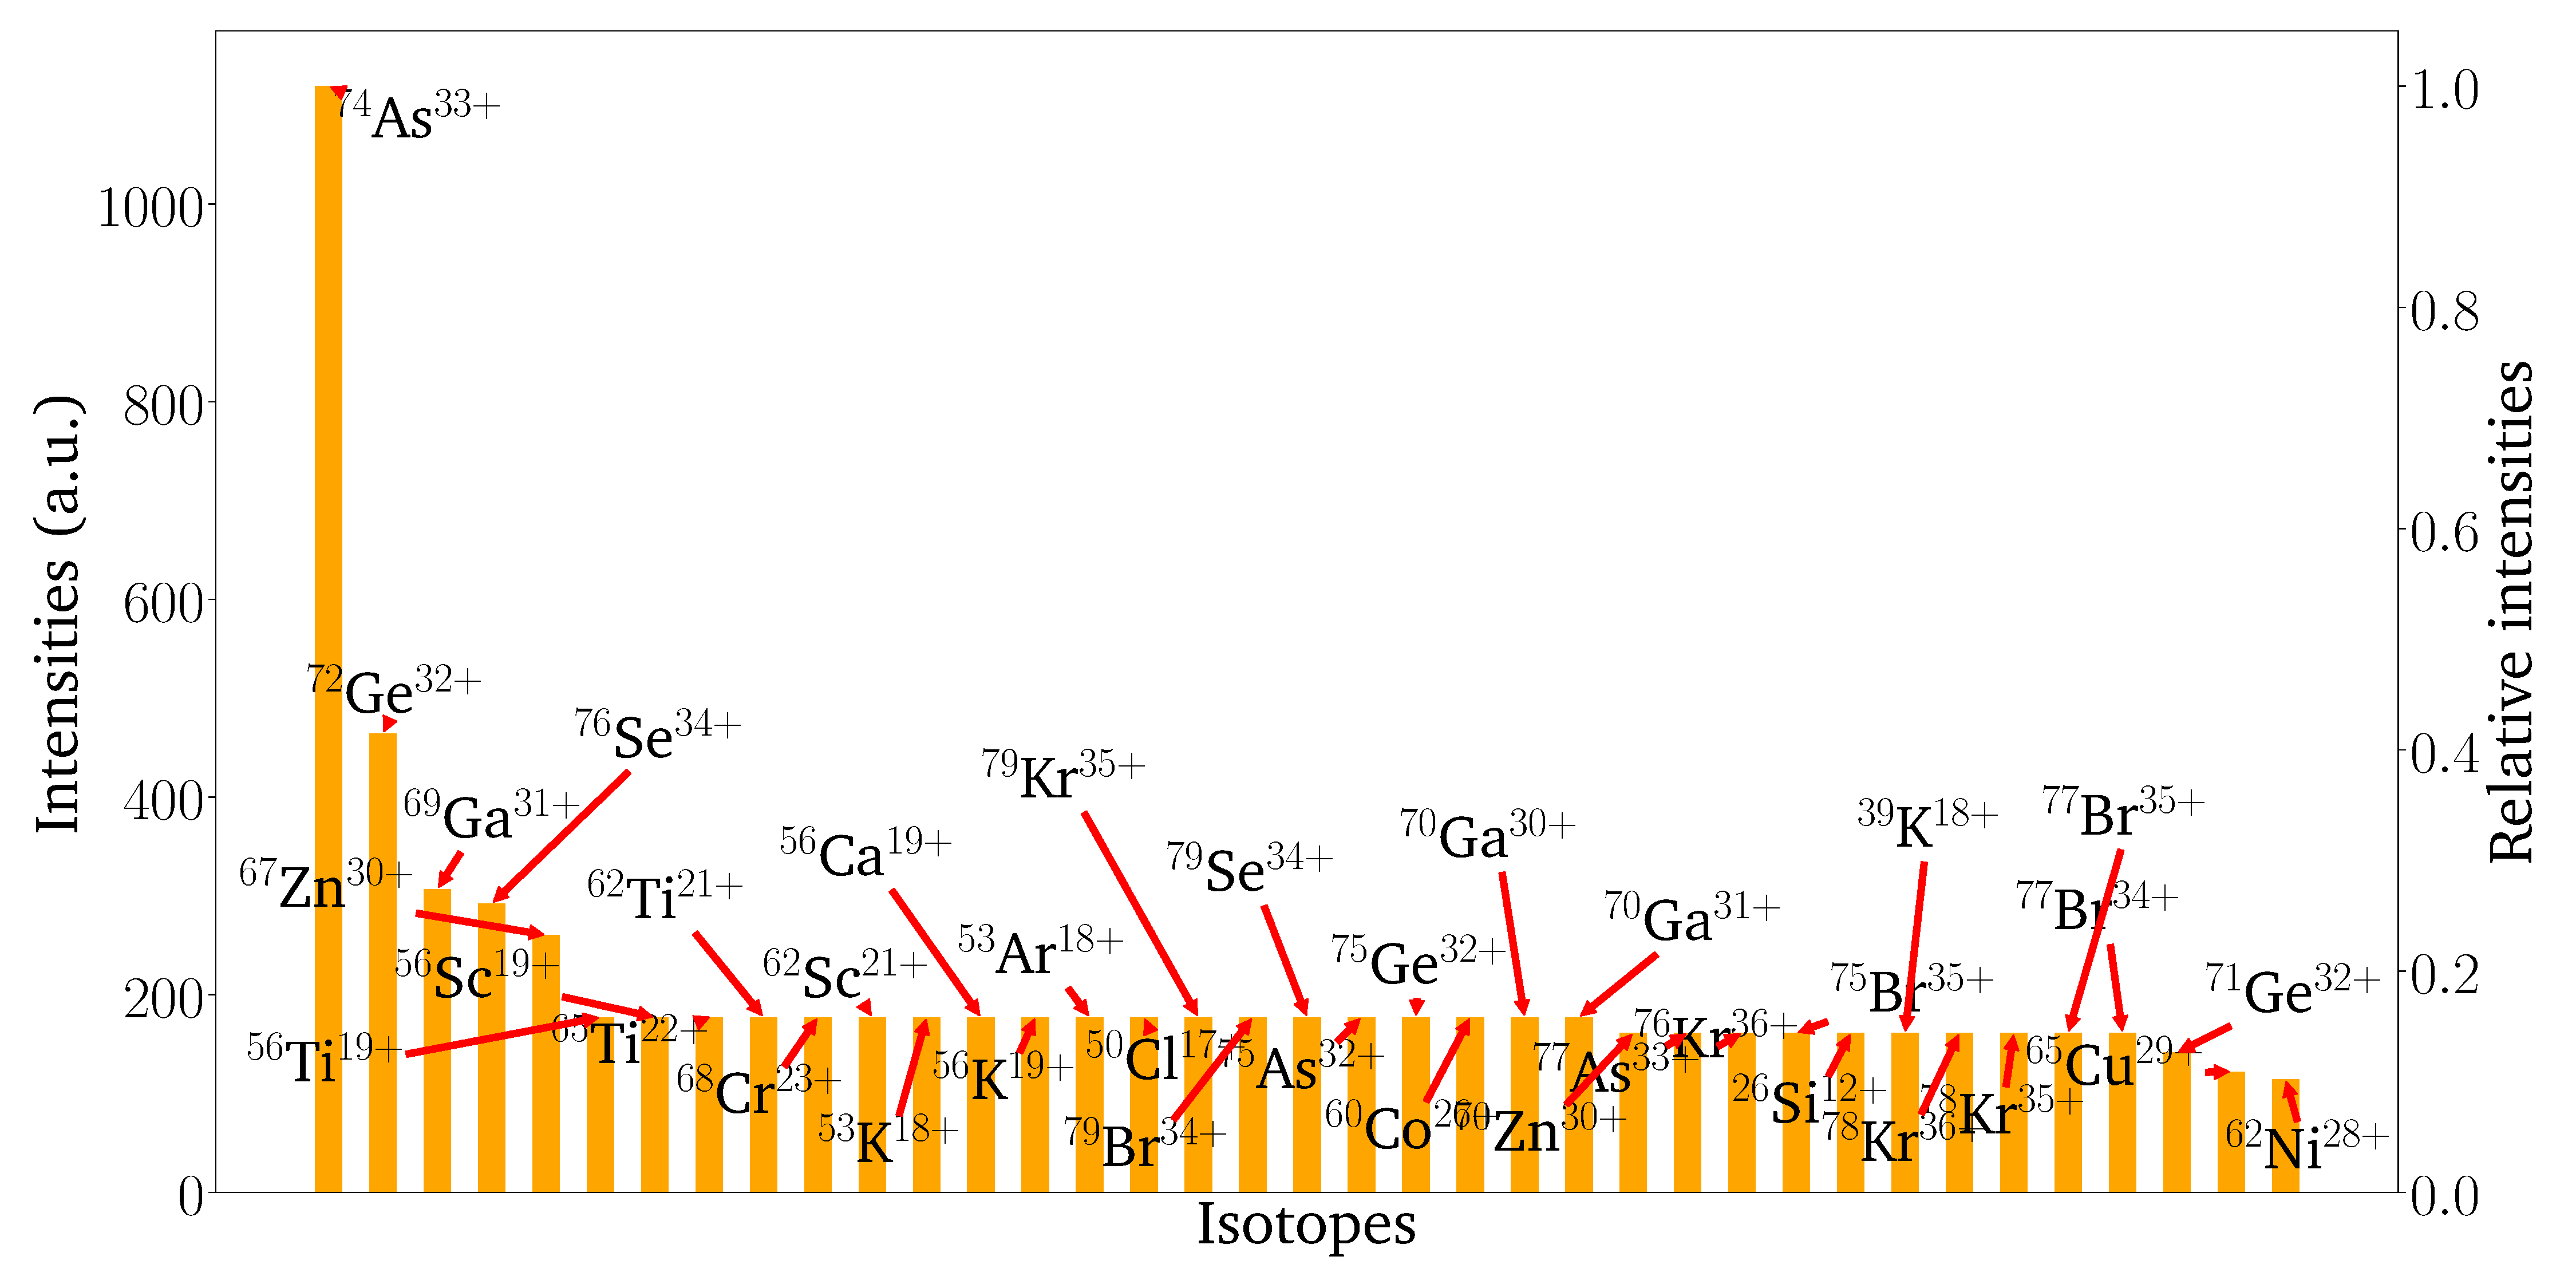
\includegraphics[width=0.76\textwidth]{72Gelise.pdf}
      \label{fig:chap3:72Ge_lise}
  }
  \vspace{0.5cm}
  \subfloat[Most expected fragments for the $^{70}\text{Se}$ setting from \textsc{LISE++} 
  calculations.]{
      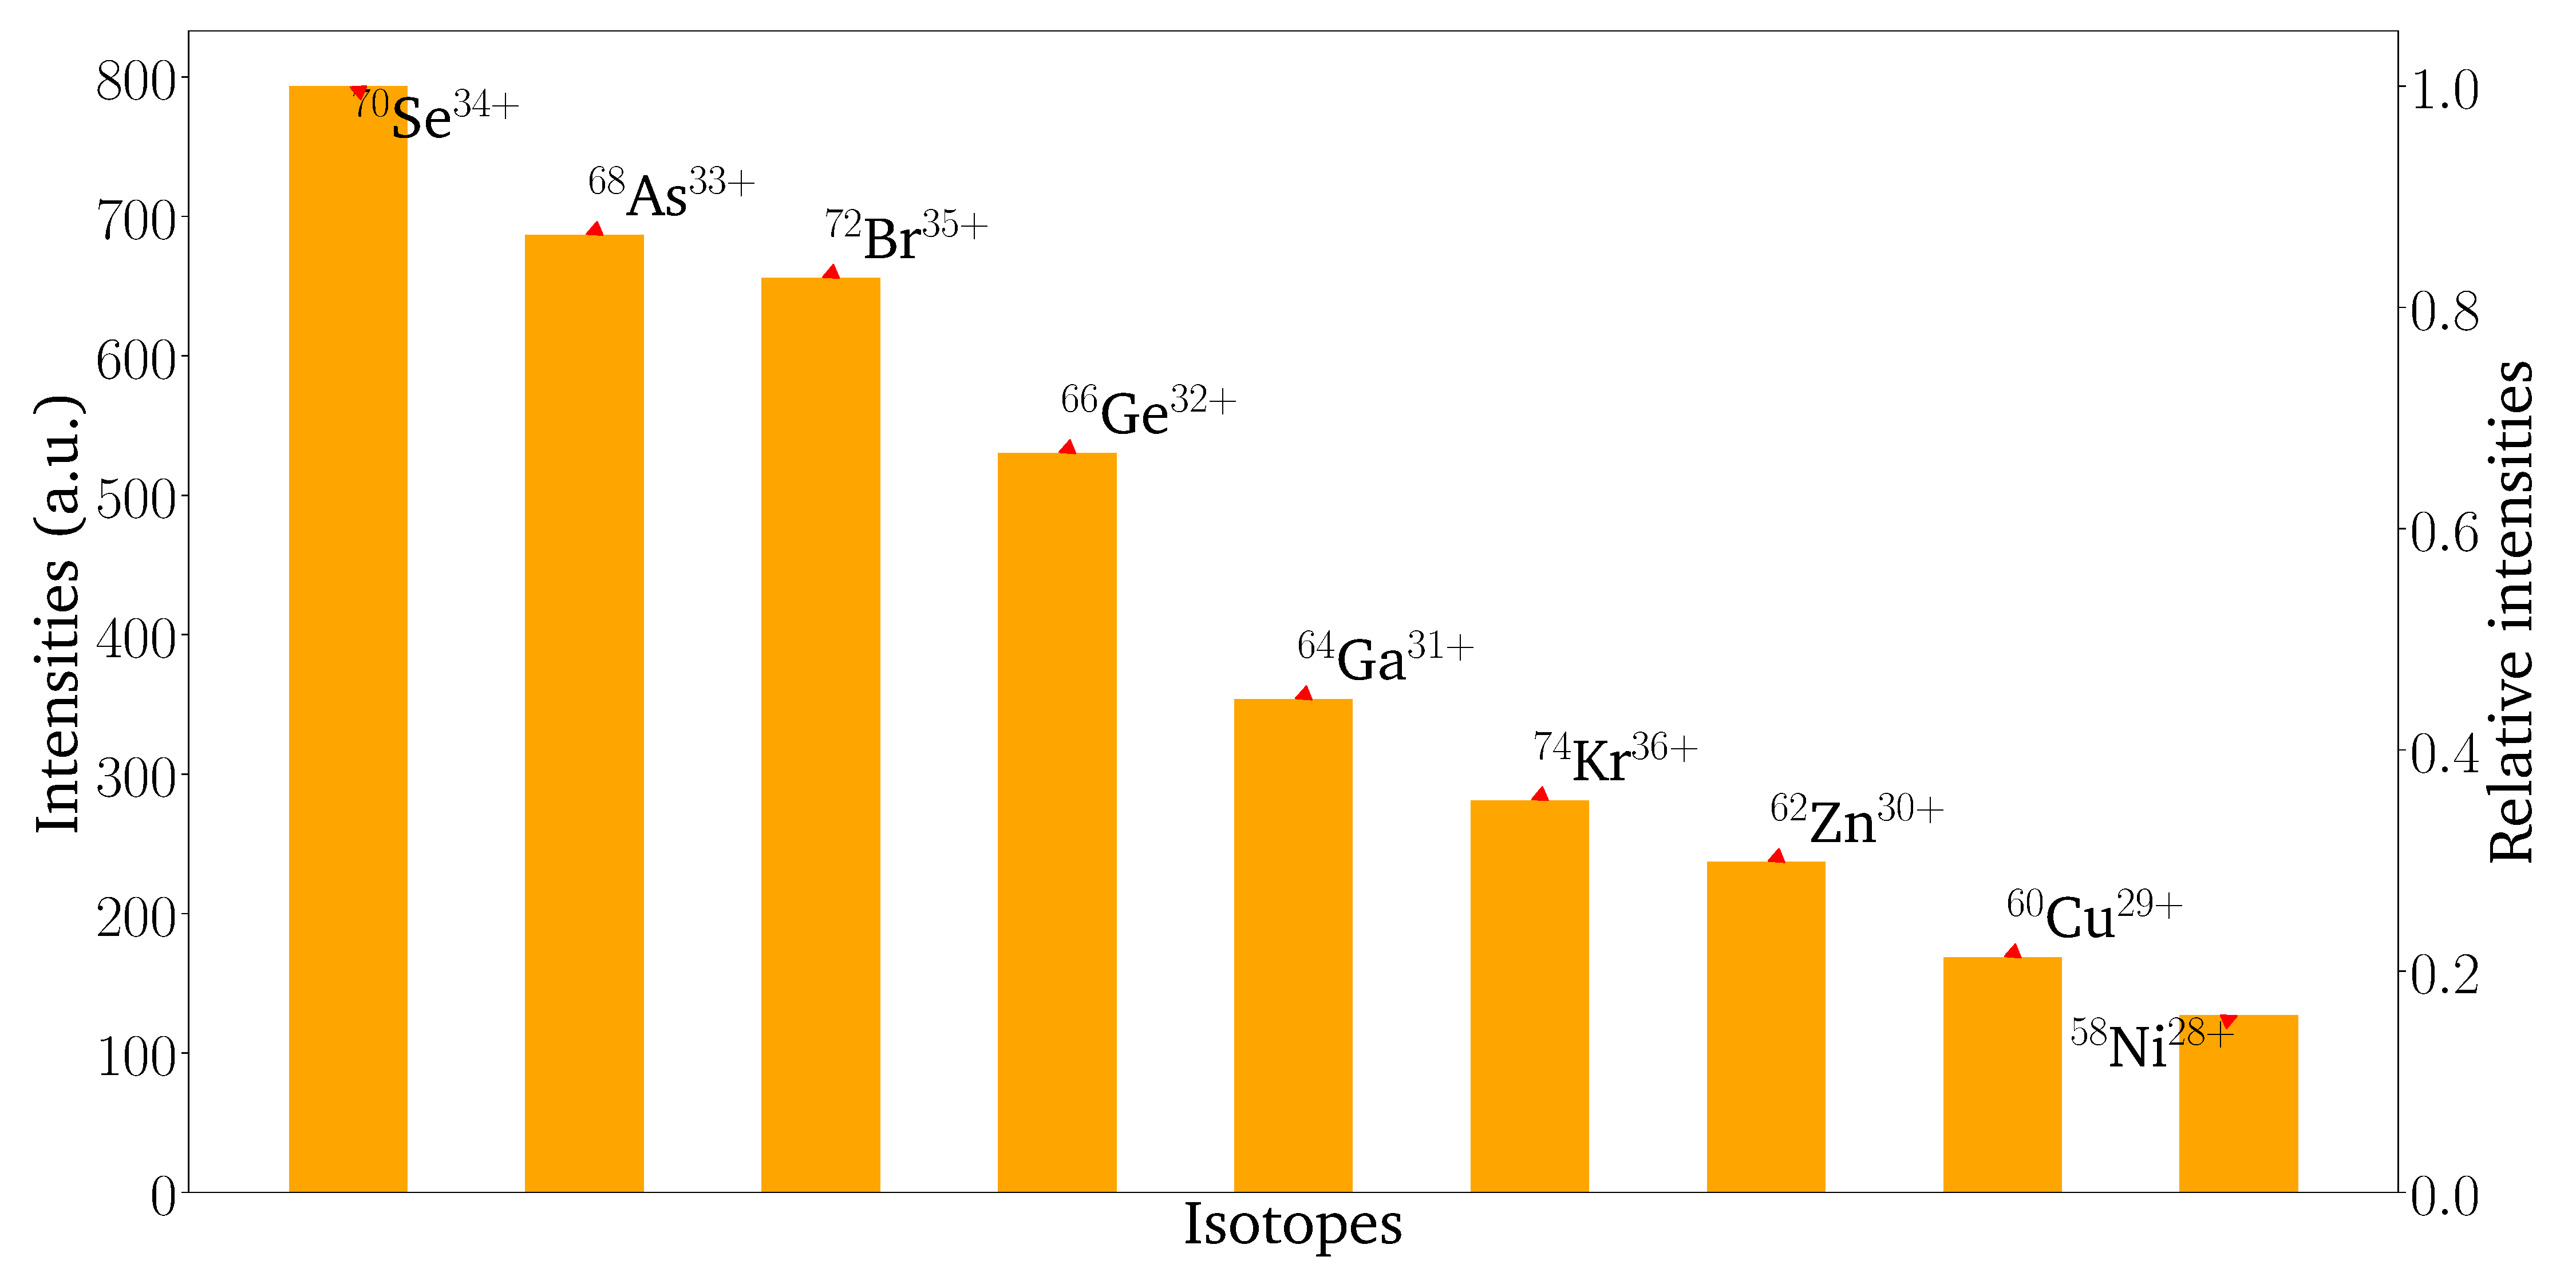
\includegraphics[width=0.76\textwidth]{70Selise.pdf}
      \label{fig:chap3:70Se_lise}
  }
  \caption{Comparison of the most expected (over $100$ arb. units of intensity) fragments from \textsc{LISE++} for each setting.}
  \label{fig:chap3:expectedfragments}
\end{figure}
\Cref{fig:chap3:ident1D} displays the broadband spectrum captured by the \textsc{NTCAP}, connected to the $245$\,MHz cavity, during the first high-resolution setting of \,\ion{72}{Ge}{32} (see \cref{sec:chap3:beamtimestory}). 
Upon examining \cref{fig:chap3:ident1D}, one of the initial observations is the presence of a consistent three-peak structure that always repeats separated by the same spacing.
By analyzing the distance between these peaks, we can determine their \textsc{eigenfrequencies} and the respective harmonic ($h$). The three ions identified, \,\ion{72}{Ge}{32}, \,\ion{74}{As}{33}, and \,\ion{76}{Se}{34}, coincide with the highest yields expected from \textsc{LISE++} (refer to \cref{fig:chap3:expectedfragments}), as illustrated in \cref{fig:chap3:72Ge_lise}.
\newpar
This (pre)identification can be realized without any prior knowledge of the ring settings, making it the initial step.
After this preliminary identification, the identified peaks are input into our identification software, \textsc{RionID}. As outlined in \cref{sec:chap3:identification}, \textsc{RionID} is based on the principle that in storage rings, the ions' revolution frequency directly correlates with their mass-to-charge ratio, as per \cref{eq:chap2:basis_i}.
Utilizing the frequency data from our pre-identified ions and using the tabulated masses \cite{AME-2020} of the expected yields (as predicted by \textsc{LISE++}), we can simulate the expected revolution frequencies of these anticipated fragments and overlay them on the experimental data as seen in \cref{fig:chap3:ident1D}.
As mentioned in \cref{subsec:chap2:identification}, discrepancies between the simulated and experimental data were observed but can be adjusted using a second-order polynomial correction as demonstrated in \cref{subsec:chap2:identification}, particularly in \cref{fig:chap2:ident_correction1} and \cref{fig:chap2:ident_correction2}.

\begin{figure}[hbt]
  \centering
  \includegraphics[width=0.95\textwidth]{1d-full-labels.png}
  \caption{Spectrum displaying revolution frequency versus amplitude from the first high-resolution setting on \,\ion{72}{Ge}{32}. The amplification curve of the $245$\,MHz detector is clearly visible. A three-peak structure has been identified and superimposed on the experimental distribution.}
  \label{fig:chap3:ident1D}
\end{figure}

Working within a narrow frequency band ($~20$\,kHz), as with the \textsc{RSAs} data (refer to \cref{subsubsec:chap2:dataacquisiton}), makes identification challenging without additional information because these repeating structures, as discussed above, are not observable in such a restricted bandwidth.
\Cref{fig:chap3:410vs245sum} presents the first high-resolution data set for \,\ion{72}{Ge}{32} in both Schottkies\footnote{Note that there is no evidence of the \,\ion{72\mathrm{m}}{Ge}{32} isomer. This absence is because the isomer has completely decayed by this time (after $1.75$\,s from injection).}.

The data, centered around the frequency of \,\ion{72}{Ge}{32}, demonstrate a clear distinction in comparison: peaks are more spread out at $410$\,MHz compared to $245$\,MHz, as expected, since the $410$\,MHz Schottky operates at a higher harmonics. Consequently, some peaks that are detected at the edges of the measured frequency range in the $245$\,MHz detector do not appear in the $410$\,MHz detector, because they fall outside its range. 
\Cref{fig:chap3:410vs245sum} also highlights the issue of \textsc{harmonic overlap}, as discussed in \cref{subsubsec:chap2:harmonicoverlapping}.
Specifically, a peak distribution visible on the right side of the center peak at $410$\,MHz, but not at $245$\,MHz, is observed. This additional peak arises from an ion with a significantly different mass-to-charge ratio, located far from the \textsc{isochronicity window}, as indicated by its \textbf{broad} and \textbf{asymmetric} shape. It was identified as coming from \,\ion{53}{Cr}{24}, but from a lower harmonic (the $125^{\mathrm{th}}$ instead of the $126^{\mathrm{th}}$).

\begin{figure}[hbt]
  \centering
  \subfloat[Spectrogram (time versus frequency) from the $245$\,MHz Schottky cavity detector. The ions identified belong to the harmonic $h=126$.]{
      \includegraphics[width=0.475\textwidth]{245vs410.png}
      \label{fig:chap3:245vs410}
  }
  \hspace{0.1cm}
  \subfloat[Spectrogram (time versus frequency) from the $410$\,MHz Schottky cavity detector. The ions identified belong to the harmonic $h=211$.]{
      \includegraphics[width=0.475\textwidth]{410vs245.png}
      \label{fig:chap3:410vs245}
  }
  \caption{Comparison of the spectrograms from the $245$\,MHz (left) and $410$\,MHz (right) detectors for the first high-resolution setting on \,\ion{72}{Ge}{32}.}
  \label{fig:chap3:410vs245sum}
\end{figure}

Following the described methodology across all different settings, I compiled all the identified ions within experiment \textsc{E143}, excluding isomers, in \cref{tab:chap3:72Geidenti} and \cref{tab:chap3:70Seidenti}. The isomers identified in each setting are presented in \cref{tab:app7:70SeIsomers} and \cref{tab:app7:72GeIsomers}. 
In the following section (\cref{sec:chap3:isochronicity}), I show the peak characteristics of each identified ion with the isochronicity curves of each setting.

\begin{table}[hbt]
  \caption{Ions identified in the high-resolution settings for \,\ion{72}{Ge}{32}, excluding isomers. The ions are arranged in increasing order of $m/q$, reading from top to bottom and left to right within the table.}
  \label{tab:chap3:72Geidenti}
  \centering
  \begin{tabular}{ccccccc}
  \toprule
  \toprule
  \,\ion{71}{Ga}{31} & \,\ion{48}{Sc}{21} & \,\ion{64}{Ni}{28} & \,\ion{73}{Ge}{32} & \,\ion{57}{Mn}{25} & \,\ion{41}{Ar}{18} & \,\ion{66}{Cu}{29} \\ 
  \,\ion{75}{Se}{33} & \,\ion{75}{As}{33} & \,\ion{50}{Ti}{22} & \,\ion{59}{Fe}{26} & \,\ion{68}{Zn}{30} & \,\ion{77}{Br}{34} & \,\ion{77}{Se}{34} \\ 
  \,\ion{43}{K}{19} & \,\ion{52}{V}{23} & \,\ion{61}{Co}{27} & \,\ion{70}{Ga}{31} & \,\ion{70}{Ge}{31} & \,\ion{72}{As}{32} & \,\ion{72}{Ge}{32} \\ 
  \,\ion{63}{Ni}{28} & \,\ion{54}{Cr}{24} & \,\ion{74}{As}{33} & \,\ion{74}{Se}{33} & \,\ion{65}{Zn}{29} & \,\ion{65}{Cu}{29} & \,\ion{56}{Mn}{25} \\ 
  \,\ion{47}{Sc}{21} & \,\ion{38}{Cl}{17} & \,\ion{76}{Se}{34} & \,\ion{67}{Ga}{30} & \,\ion{67}{Zn}{30} & \,\ion{58}{Fe}{26} & \,\ion{49}{Ti}{22} \\ 
  \,\ion{69}{Ga}{31} & \,\ion{40}{Ar}{18} & \,\ion{60}{Co}{27} & \,\ion{71}{Ge}{32} & \,\ion{51}{V}{23} & \,\ion{62}{Ni}{28} & \,\ion{73}{As}{33} \\ 
  \,\ion{42}{K}{19} & \,\ion{53}{Cr}{24} & \,\ion{64}{Cu}{29} & \,\ion{33}{P}{15} & \,\ion{44}{Ca}{20} & \,\ion{66}{Zn}{30} & \,\ion{55}{Mn}{25} \\ 
  \,\ion{68}{Ga}{31} & \,\ion{57}{Fe}{26} & \,\ion{46}{Sc}{21} & \,\ion{59}{Co}{27} & \,\ion{48}{Ti}{22} & \,\ion{61}{Cu}{28} & \,\ion{61}{Ni}{28} \\ 
  \,\ion{37}{Cl}{17} & \,\ion{50}{V}{23} & \,\ion{63}{Cu}{29} & \,\ion{39}{Ar}{18} & \,\ion{52}{Cr}{24} & \,\ion{54}{Mn}{25} & \,\ion{41}{K}{19} \\ 
  \,\ion{56}{Fe}{26} & \,\ion{43}{Ca}{20} & \,\ion{30}{Si}{14} & \,\ion{45}{Sc}{21} & \,\ion{47}{Ti}{22} & \,\ion{32}{P}{15} & \,\ion{34}{S}{16} \\
  \,\ion{76}{Kr}{36} & & & & & & \\
  \bottomrule
  \bottomrule
  \end{tabular}
\end{table}

\begin{table}[hbt]
  \caption{Ions identified in the high-resolution settings for \,\ion{70}{Se}{34}, excluding isomers. The ions are arranged in increasing order of $m/q$, reading from top to bottom and left to right within the table.}
  \label{tab:chap3:70Seidenti}
  \centering
  \begin{tabular}{ccccccc}
  \toprule
  \toprule
  \,\ion{45}{Sc}{21} & \,\ion{47}{Ti}{22} & \,\ion{32}{P}{15} & \,\ion{49}{V}{23} & \,\ion{34}{S}{16} & \,\ion{51}{Cr}{24} & \,\ion{53}{Mn}{25} \\
  \,\ion{36}{Cl}{17} & \,\ion{55}{Fe}{26} & \,\ion{38}{Ar}{18} & \,\ion{57}{Co}{27} & \,\ion{59}{Ni}{28} & \,\ion{40}{K}{19} & \,\ion{61}{Cu}{29} \\
  \,\ion{42}{Ca}{20} & \,\ion{63}{Zn}{30} & \,\ion{65}{Ga}{31} & \,\ion{67}{Ge}{32} & \,\ion{69}{As}{33} & \,\ion{46}{Ti}{22} & \,\ion{71}{Se}{34} \\
  \,\ion{48}{V}{23} & \,\ion{73}{Br}{35} & \,\ion{75}{Kr}{36} & \,\ion{50}{Cr}{24} & \,\ion{77}{Rb}{37} & \,\ion{52}{Mn}{25} & \,\ion{27}{Al}{13} \\
  \,\ion{54}{Fe}{26} & \,\ion{56}{Co}{27} & \,\ion{29}{Si}{14} & \,\ion{58}{Ni}{28} & \,\ion{60}{Cu}{29} & \,\ion{62}{Zn}{30} & \,\ion{64}{Ga}{31} \\
  \,\ion{33}{S}{16} & \,\ion{66}{Ge}{32} & \,\ion{68}{As}{33} & \,\ion{70}{Se}{34} & \,\ion{72}{Br}{35} & \,\ion{74}{Kr}{36} & \,\ion{39}{K}{19} \\
  \,\ion{43}{Sc}{21} & \,\ion{45}{Ti}{22} & \,\ion{47}{V}{23} & \,\ion{49}{Cr}{24} & \,\ion{53}{Fe}{26} & \,\ion{55}{Co}{27} & \,\ion{57}{Ni}{28} \\
  \,\ion{59}{Cu}{29} & \,\ion{61}{Zn}{30} & \,\ion{63}{Ga}{31} & & & & \\
  \bottomrule
  \bottomrule
  \end{tabular}
  \end{table}

%  \iffalse
%\fi
\section{Isochronicity curves}\label{sec:chap3:isochronicity}

In this section, for each identified ion in the high-resolution settings (refer to \cref{sec:chap3:identification}), we determine its spectral characteristics, including the frequency centroid and standard deviation, using Gaussian fitting. After filtering out the identified ion with lower signal-to-noise ratio, due to having low statistics or/and being located outside the resonance region of the detector, we plot the variation of the peak's spread as a function of revolution time. Following this, we perform a fit in accordance with \cref{eq:chap2:sigma_T_final}. The reduced $\chi^2$ was $\sim1$ for each fit, ensuring the reliability of the results of the fit. Through this analysis, we gain insights into the isochronicity condition and the settings of the ring, as previously described in \cref{subsec:chap2:isocurve}. The results of each of the isochronicity curves displayed in \cref{fig:chap3:iso72Ge1}, \cref{fig:chap3:iso72Ge2}, \cref{fig:chap3:iso70SeMay} and \cref{fig:chap3:iso70SeJune} are compiled in \cref{tab:chap3:iso_fit_parameters}.

\begin{figure}[hbt]
  \centering
  \includegraphics[width=1\textwidth]{72Ge_1st_isocurve.png}
  \caption{Isochronicity curve of the first high-resolution setting achieved on \,\ion{72}{Ge}{32}, which is highlighted within the green box. See discussion in \cref{sec:chap3:isochronicity}.}
  \label{fig:chap3:iso72Ge1}
  \end{figure}
  
  \begin{figure}[hbt]
  \centering
  \includegraphics[width=1\textwidth]{72Ge_2nd_isocurve.png}
  \caption{Isochronicity curve of the second high-resolution setting achieved on \,\ion{72}{Ge}{32}, which is highlighted within the green box. See discussion in \cref{sec:chap3:isochronicity}.}
  \label{fig:chap3:iso72Ge2}
  \end{figure}

When comparing both settings for \,\ion{72}{Ge}{32}, it can be observed that the minimum spread achievable ($\sigma_{\mathrm{sys}}$) is quite similar across both settings, indicating that the maximum mass resolving power (refer to \cref{sec:chap3:massresolvingpower}) was similar. Also, both $\gamma_t$ are nearly the same, indicating that each setting was optimized for nearly the same $m/q$. The significant distinction, however, lies in the rate of isochronicity loss, enveloped in $\sigma_p / p$, which is higher in the first setting ($ 0.283(3)$~\%) compared to the second one ($ 0.149(1)$~\%). This difference is attributed to the use of a closer scraper setting in the second setting, as mentioned in \cref{sec:chap3:beamtimestory} and described in \cref{subsec:chap2:isocurve}. 
By narrowing the allowed momentum space, we reduce the variations in the $\gamma_t$ as a function of the orbits and diminish yield asymmetries, as shown in \cref{fig:chap2:brhocut}. Consequently, we ensure that across the ring's entire acceptance, the peaks appear more symmetric and are less pronounced. However, this comes with a trade-off: lower statistics since we are intercepting the beam; we are removing ions.


In comparing the settings across the experiment, the transition energy factor, $\gamma_t$, is generally kept constant, since at the \textsc{ESR} is preferred to fix ion-optical parameters and tune the $\gamma$ of the ions to match $\gamma_t$. This is not true in the first setting for \,\ion{70}{Se}{34}, where a significant deviation in $\gamma_t$ is observed, however the $\gamma$ were not adjusted accordingly\footnote{This was because the behavior of the \textsc{S+IMS} was not fully understood at the time. Now, it should be straightforward.}. In addition, the $\sigma_p / p$~(\%) values are almost the same as in the first setting of \,\ion{72}{Ge}{32}. This similarity is because the measurements for \,\ion{70}{Se}{34} were taken right after those for \,\ion{72}{Ge}{32}, as mentioned in \cref{sec:chap3:beamtimestory}, without adjusting the scraper positions.
Consequently, the isochronous condition was not set on \,\ion{70}{Se}{34} but in a different $m/q$ region, as shown in \cref{fig:chap3:iso70SeMay}. Furthermore, the parameters for the second setting align well with those of the high-resolution settings for \,\ion{72}{Ge}{32}. In contrast, the first setting for \,\ion{70}{Se}{34} presents the lowest mass resolving power of all settings evaluated, reflected in the highest $ \sigma_{\mathrm{sys}} = 0.33 (2) $~(ps) value.

\begin{table}[hbt]
\caption{Parameters obtained from fitting the isochronicity curve for each setting.}
\label{tab:chap3:iso_fit_parameters}
\centering
\begin{tabular}{cccc}
\toprule
\toprule
\textsc{Setting}             & $\gamma_t$      & $\sigma_p / p$~(\%) & $\sigma_{\mathrm{sys}}$~(ps) \\
\midrule\midrule
\,\ion{72}{Ge}{32} ($1$)  &   $1.3959 (1)  $   & $ 0.283 (3)$          &  $ 0.12 (2) $ \\
\,\ion{72}{Ge}{32} ($2$) &   $1.3956 (1) $   & $ 0.149 (1)$          &    $ 0.143 (7)$  \\
\,\ion{70}{Se}{34} ($1$)  &   $1.3784 (1)  $   & $ 0.283 (4)$          &  $ 0.33 (2) $ \\
\,\ion{70}{Se}{34} ($2$) &   $1.3950 (3)  $   & $ 0.109 (8)$          &  $ 0.161 (6)$ \\
\bottomrule
\bottomrule
\end{tabular}%
\end{table}

The experimental values used in the previous figures are compiled in \cref{apdx:tables}, in \cref{tab:app7:72Ge2ndI}, \cref{tab:app7:72Ge2ndII}, \cref{tab:app7:72Ge1stI}, \cref{tab:app7:72Ge1stII}, \cref{tab:app7:70Se1stI}, \cref{tab:app7:70Se1stII}, \cref{tab:app7:70Se2nd}.

These isochronicity curves serve as a fundamental understanding of the \textsc{S+IMS}. Moreover, they can be connected to the mass resolving power that is achieved. This is further discussed in \cref{sec:chap3:massresolvingpower}.

\begin{figure}[hbt]
\centering
\includegraphics[width=1\textwidth]{70Se_may_isocurve.png}
\caption{Isochronicity curve of the first high-resolution setting on \,\ion{70}{Se}{34}, which is highlighted within the green box. See discussion in \cref{sec:chap3:isochronicity}.}
\label{fig:chap3:iso70SeMay}
\end{figure}
  
\begin{figure}[hbt]
\centering
\includegraphics[width=1\textwidth]{70Se_june_isocurve.png}
\caption{Isochronicity curve of the high-resolution setting on \,\ion{70}{Se}{34}, which is highlighted within the green box. See discussion in \cref{sec:chap3:isochronicity}.}
\label{fig:chap3:iso70SeJune}
\end{figure}

  %\fi
  %\iffalse
  %\iffalse
\section{Mass resolving power}\label{sec:chap3:massresolvingpower}
From the isochronicity curves discussed in \cref{sec:chap3:isochronicity}, we can convert the frequency (time) spreads ($\sigma_f$ or $\sigma_T$) into spreads in mass, and subsequently into mass resolving power ($R$) and the minimum resolvable peak width at full width at half maximum (\textsc{FWHM}). According to \cref{eq:intro:basic}, for isochronous ions $\gamma \rightarrow \gamma_t$, simplifying \cref{eq:intro:basic} into:

\begin{equation}
\frac{\Delta{f}}{f}=-\frac{1}{\gamma_t^2}\frac{\Delta(m/q)}{m/q}.
\label{eq:chap3:basic_iso_particles}
\end{equation}

Therefore, defining the resolving power at \textsc{FWHM} as:
\begin{equation}
      R = \frac{m}{\Delta m} = \frac{1}{\gamma_t^2} \frac{f}{2\sqrt{2\ln(2)}\sigma_f},
\end{equation}
  where $f$ is the revolution frequency and $\sigma_f$ the standard deviation of the peak in frequency.
  For the ground state of \,\ion{72}{Ge}{32} in the second setting, we predict:
  \begin{equation}
      R  = \frac{1}{(1.396)^2} \frac{243105253.5}{2\sqrt{2\ln(2)}58.2} \approx 9.1 \times 10^5.
  \end{equation}
  This represents the \textbf{highest mass resolving power} reported so far in \textsc{IMS}.
  It enables us to differentiate an isomeric state in \,\ion{72}{Ge}{32} with a mass difference (or excitation energy) at \textsc{FWHM} of:
  \begin{equation}
    \Delta m = m(^{72}\mathrm{Ge}^{32+}) / R \approx \bm{74}\,\mathrm{\bf keV}.
  \end{equation}

  \begin{figure}[hbt]
    \centering
    \includegraphics[width=0.3\linewidth]{72br_iso_sketch.png}
    \caption{A sketch of the \,\isomer{72}{Br}$^{35+}$, along with some of its nuclear properties (in the absence of electrons).}
    \label{fig:chap3:72mbr_sketch}
  \end{figure}

  However, \,\ion{72}{Ge}{32} lacks an isomer with this specific excitation energy, preventing us from validating this remarkable prediction experimentally. Nonetheless, the high-resolution settings for \,\ion{70}{Se}{34} do include \,\ion{72}{Br}{35}. 

  \begin{figure}[hbt]
    \centering
    \includegraphics[width=0.95\textwidth]{72mBr_1to1_4.png}
    \caption{(Top) Decay of a single particle of \,\ion{72\mathrm{m}}{Br}{35} in the isomeric state to  a single particle of \,\ion{72\mathrm{g}}{Br}{35} in the ground state. The excitation of the isomer  is $101$\,keV. (Bottom) The areas of the corresponding single particles and background. (Left) Projection on the frequency axis containing the equivalence between frequency and energy.}
   \label{fig:chap3:72mBr1to1}
  \end{figure}

  \,\isotope{72}{Br} has an isomer with energy $100.76(15)$\,keV \cite{ENSDF} and a half-life of $10.6(3)$\,s \cite{ENSDF} in its neutral state. Therefore, in terms of half-life we should observe it.
  Performing the same calculation as for \,\ion{72}{Ge}{32}, for \,\ion{72}{Br}{35} within the second high-resolution setting of \,\ion{70}{Se}{34}, we deduce a resolving power of $R \approx 6.3\cdot10^5$, allowing us to, in principle, resolve a $\Delta m \approx 106$\,keV isomeric state (assuming it is produced and stored within the ring). This prediction was confirmed by a clear separation of the isomeric and ground state, visible in \cref{fig:chap3:72mBr1to1} and \cref{fig:chap3:72mBrproject}. This demonstrates that we can use the isochronicity curve to measure and monitor the ion-optical parameters, while tuning the ring settings with the goal of improving our resolving power.

  \begin{figure}[hbt]
  \centering
  \includegraphics[width=0.85\textwidth]{72mbr-prooject2.png}
  \caption{Sum of $11$ spectrograms (injections), from the $410$\,MHz detector, containing both the ground and isomeric states of \,\ion{72}{Br}{35}. (Top) Projection of the spectrogram on the frequency axis, highlighting the resolution of the peaks. Between brackets can be found the time (y-axis) and frequency (x-axis) resolutions.}
  \label{fig:chap3:72mBrproject}
  \end{figure}

  When we move out of the \textsc{isochronous window}, the relation described in \cref{eq:chap3:basic_iso_particles} is no longer true; the second term in \cref{eq:intro:basic} starts to influence, leading to broader peaks. Consequently, this leads to a decrease in resolving power. The rate of deterioration is related to the $\sigma_p/p$ ratio, as already described in \cref{sec:chap3:isochronicity}. 

%\fi

\section{Mass measurements}\label{sec:chap3:massmeasurements}

Mass measurements were conducted using the polynomial fitting method detailed in \cref{subsec:chap2:massdetermination}, applied to the ions depicted in the isochronicity curves from \cref{sec:chap3:isochronicity}. This section presents the calculated masses.

\Cref{fig:chap3:mass72Ge1} and \cref{fig:chap3:mass72Ge2} show the difference between the measured masses and the tabulated values. Given that all the ions are close to the valley of stability, their masses have already been measured with high-precision elsewhere. Consequently, they can be used as references. The methodology used for mass determination, as outlined in \cref{subsec:chap2:massdetermination}, involves a fitting procedure considering all ions. However, ions located further from the isochronicity point are measured with less precision and contribute the most to the overall uncertainty affecting all measured ions. To achieve a reduced $\chi^2$ value of $1$, an additional systematic uncertainty of approximately $9$\,keV must be accounted for.
\newpar
All the measured masses agree well within uncertainties with the \textsc{AME} data \cite{AME-2020}, except one, \,\ion{72}{As}{32}, which deviates by more than $3\sigma$ in both \,\ion{72}{Ge}{32} settings (see the orange boxes in \cref{fig:chap3:mass72Ge1} and \cref{fig:chap3:mass72Ge2}). A recent study (after \textsc{AME$2020$}), reports a similar downward shift in mass for \,\isotope{72}{As}, with a measured deviation of $12.4(40)$\,keV \cite{PhysRevC.103.065502} at \textsc{JYFLTRAP}, which aligns with our findings within $1.8\sigma$.
The results, including the newly measured values (highlighted in a green row), are tabulated in \cref{tab:app7:72GeCMM1st} and \cref{tab:app7:72GeCMM2nd}.

  \begin{figure}
    \centering
    \includegraphics[width=0.95\textwidth]{72Ge_1st_mass.png}
    \caption{Deviation of the mass measurements from the values tabulated in \textsc{AME$2020$} \cite{AME-2020}, using the first high-resolution setting achieved on \,\ion{72}{Ge}{32}. Inside the orange box is illustrated the improved mass. The improved mass measurement is depicted within the orange box. See discussion in \cref{sec:chap3:massmeasurements}.}
    \label{fig:chap3:mass72Ge1}
  \end{figure}
    
  \begin{figure}
    \centering
    \includegraphics[width=0.95\textwidth]{72Ge_2nd_mass.png}
    \caption{Deviation of the mass measurements from the values tabulated in \textsc{AME$2020$} \cite{AME-2020}, using the second high-resolution setting achieved on \,\ion{72}{Ge}{32}. The improved mass measurement is depicted within the orange box. See discussion in \cref{sec:chap3:massmeasurements}.}
    \label{fig:chap3:mass72Ge2}
  \end{figure}
    
  For the first setting on \,\ion{70}{Se}{34}, we again notice a measurement that significantly differs from the \textsc{AME} values, highlighted in the light-orange row of \cref{tab:app7:70SeCMMmay} and in the orange box of \cref{fig:chap3:mass70SeMay}. Specifically, \,\ion{69}{As}{33} is listed in \textsc{AME2020} \cite{AME-2020} with an uncertainty of $30$\,keV. Recently, this isotope's mass was directly measured for the first time at the \textsc{FRS@GSI} using \textsc{MR-TOF-MS}, achieving a lower uncertainty of $22$\,keV \cite{PhysRevC.103.034319}. Their value falls within $1.3\sigma$ of ours, yet our measurement presents $\sim9$\,keV of uncertainty, which is more than a half lower.
  The details of this measurement are tabulated in \cref{tab:app7:70SeCMMmay}.

    \begin{figure}
    \centering
    \includegraphics[width=0.95\textwidth]{70Se_may_massexcess.png}
    \caption{Deviation of the mass measurements from the values tabulated in \textsc{AME$2020$} \cite{AME-2020}, using the first high-resolution setting on \,\ion{70}{Se}{34}. The improved mass measurement is depicted within the orange box. See discussion in \cref{sec:chap3:massmeasurements}.}
    \label{fig:chap3:mass70SeMay}
    \end{figure}
    
    Finally, in the second setting on \,\ion{70}{Se}{34}, due to low statistics we do not have as many ions stored than in the previous settings, and we do not observe any interesting results. Its results are tabulated in \cref{tab:app7:70Se1stII}.
    \begin{figure}
    \centering
    \includegraphics[width=0.95\textwidth]{70Se_june_massexcess.png}
    \caption{Deviation of the mass measurements from the values tabulated in \textsc{AME$2020$} \cite{AME-2020}, using high-resolution setting on \,\ion{70}{Se}{34}.}
    \label{fig:chap3:mass70SeJune}
    \end{figure}
    
  \subsection{Determination of the excitation energy of \,\ion{72\mathrm{m}}{Ge}{32}}\label{subsec:chap3:72gemeasurementenergy}
  \textit{\footnotesize Part of the text, figures and tables within this subsection have already been submitted for publication to Physical Review Letters in D. Freire-Fernandez et al., Measurement of the Isolated Nuclear Two-Photon Decay in $^{72}\mathrm{Ge}$ (2024) \cite{freirefernández2023measurement}}.

  The measured frequencies and precisely known mass of $^{72}\mathrm{Ge}^{32+}$\,\cite{AME-2020}, allowed us to independently determine the excitation energy of the isomeric state via \cref{eq:chap2:isomer_energy}, using the method described in \cref{subsubsec:chap2:excitationenergydeter}.
  Data from both \textsc{RSAs} and for both settings ($1$,$2$) were analyzed separately.
  The results are listed in \cref{tab:chap3:isomer_energy}.
  All obtained $\omega_0$ values are in good agreement with the tabulated excitation energy \cite{ENSDF}.
  
  \begin{table}[hbt]
    \caption{Measured frequency difference $\Delta f$ between the isomeric and ground state and the deduced excitation energy $\omega_0$ of the isomer for the two different data subsets ($i$) in each Schottky detector. The last column corresponds to the weighted average of the values obtained with each detector.}
    \label{tab:chap3:isomer_energy}
    \centering
    \begin{tabular}{ccccc} 
      \toprule 
      \toprule
      \textsc{Detector} & $i$ & $\Delta f$ (Hz) & $\omega_0$ (keV) & \multicolumn{1}{c}{$\overline{\omega_{0}}$ (keV)}\\
      \midrule\midrule
      \multirow{2}{*}{\textsc{SD}$_{410}$} & $1$ & $2162\left(8\right)$ & $694.4\left(31\right)$ & \multirow{2}{*}{$692.8\left(19\right)$} \\ \cline{2-4}
      & $2$ & $2157\left(4\right)$ & $691.8\left(24\right)$ & \\
      \multirow{2}{*}{\textsc{SD}$_{245}$} & $1$ & $1301\left(7\right)$ & $699.7\left(43\right)$ & \multirow{2}{*}{$695.0\left(32\right)$} \\ \cline{2-4}
      & $2$ & $1290\left(4\right)$ & $692.8\left(29\right)$ & \\
      \bottomrule
      \bottomrule
    \end{tabular}
    
  \end{table}
%\iffalse

\section{Half-life measurements}\label{sec:chap3:halflifemeasurements}
  %Here I show the different half-lives measured during the experiment, treating each case individually.
  %\iffalse 

  \subsection{Nuclear two-photon decay in \,\isotope{72}{Ge}}\label{subsec:chap3:hl-twophoton}
  \textit{\footnotesize Part of the text, figures and tables within this subsection have already been submitted for publication to Physical Review Letters in D. Freire-Fernandez et al., Measurement of the Isolated Nuclear Two-Photon Decay in $^{72}\mathrm{Ge}$ (2024) \cite{freirefernández2023measurement}}.

  As previously discussed in \cref{sec:chap1:twophotonstorage}, \,\isotope{72}{Ge} is one of the few nuclides known with a ground and first (low-lying) excited states having $J^\pi = 0^{+}$. Consequently, single-photon decay (\cref{subsubsection:intro:gammadecay}) and \textsc{IPC} (\cref{subsubsection:intro:internalpaircreation}) are not allowed. In its atomic form (in the presence of electrons), the isomer decays to the ground state via \textsc{IC} (\cref{subsubsection:intro:internalconversion}) with a half-life of $444.2\left(8\right)$\,ns~\cite{BRAUN1984}. However, when all electrons are removed, this decay mode is also forbidden, allowing for the observation of the rare nuclear two-photon decay (see \cref{chap:100years}). The properties of this nuclide and its decay process are represented in \cref{tab:chap3:72geproperties} and sketched in \cref{fig:chap3:sketch72ge}, respectively.
  \begin{table}[hbt]
    \centering
    \captionof{table}{Nuclear properties of the ground ($^{\mathrm{g}}$) and first excited ($^{\mathrm{m}}$) state of \,\isotope{72}{Ge}.}
    \label{tab:chap3:72geproperties}
      %\resizebox{\columnwidth}{!}{
      \begin{tabular}{ccccc}
      \toprule
      \toprule
      \textsc{Nuclide}                        & \textsc{Energy} (keV)  & $J^{\pi}$ & $T_{1/2}$ (ns) & \textsc{Decay mode} \\ 
      \midrule\midrule
      $^{72\mathrm{g}}\mathrm{Ge}$ & $0$            & $0^+$  & Stable & None \\
      $^{72\mathrm{m}}\mathrm{Ge}$  & $691.43(4)$~\cite{ENSDF}    & $0^+$  & $444.2(8)$~\cite{BRAUN1984} & $E0$ \\
      \bottomrule
      \bottomrule
      \end{tabular}
      %}
  \end{table}

  \begin{figure}[hbt]
    \centering
    \includegraphics[width=0.45\linewidth]{72ge_iso_sketch.png}
    \caption{Sketch of the nuclear two-photon decay of \,\ion{72}{Ge}{32} in the absence of electrons.}
    \label{fig:chap3:sketch72ge}
  \end{figure}

The trace of the isomer \,$^{72\mathrm{m}}\mathrm{Ge}^{32+}$ in \cref{fig:chap3:single} corresponds to an injection with initially three \,$^{72\mathrm{m}}\mathrm{Ge}^{32+}$ particles.
Injections containing up to three \,$^{72\mathrm{m}}\mathrm{Ge}^{32+}$ particles were observed in the first subset of data (comprising $103$ injections). In contrast, in the second subset this number is reduced approximately by half, while we recorded $17$ times longer, therefore reaching higher statistics. More details were given in \cref{sec:chap3:beamtimestory}.
\newpar
To determine the half-life of \,$^{72\mathrm{m}}\mathrm{Ge}^{32+}$ (fully-stripped\footnote{Note that this is equivalent to determining the (partial) half-life of the nuclear two-photon decay, as we are studying fully-stripped ions, as depicted in \cref{fig:chap3:sketch72ge}.}), all spectra measured by both \textsc{RSAs} were adjusted in frequency (see \cref{subsubsec:chap2:freqcorrection}) by setting the center of the $^{72\mathrm{g}}\mathrm{Ge}$ peaks to $0$\,Hz.
Afterwards, the spectra were summed up separately for each \textsc{RSA} and data subset.
The resultant combined spectra of the $410$\,MHz detector during setting $1$ and $2$ are shown in \cref{fig:chap3:combined} and \cref{fig:chap3:spect4102}, respectively.
Once summed all the spectrograms, we monitor the frequency region corresponding to the isomeric state over time, as previously discussed in \cref{subsec:chap2:halflifedetermination}.

\begin{figure}[hbt]
  \centering
  \includegraphics[width=0.85\textwidth]{single_label_2p.png}
  \caption{Time after injection ($\delta t=9.22$\,ms per time bin) versus revolution frequency ($\delta f=108$\,Hz per frequency bin) spectrogram of a single injection from setting $1$ centered on $^{72\mathrm{g}}\mathrm{Ge}^{32+}$ from $0$ to $300$\,ms. The power spectral density of each ion species is proportional to their ion number (\cref{eq:chap2:schottkyI}).}
  \label{fig:chap3:single}
\end{figure}

\begin{figure}[hbt]
  \centering
  \includegraphics[width=0.85\textwidth]{combined_2p.png}
  \caption{Frequency spectrogram of the sum of $102$ single injections such as the one in \cref{fig:chap3:single}.}
  \label{fig:chap3:combined}
\end{figure}

\begin{figure}[hbt]
  \centering
  \includegraphics[width=0.85\textwidth]{spectrogram_s2_410.png}
  \caption{Frequency spectrogram of the sum of $2459$ injections of the second-achieved high-resolution setting measured with the $410$\,MHz Schottky cavity. The region used for analyzing the half-life of $^{72\mathrm{m}}\mathrm{Ge}^{32+}$ is highlighted in red.}
  \label{fig:chap3:spect4102}
\end{figure}

The decrease in intensity of the $^{72\mathrm{m}}\mathrm{Ge}^{32+}$ trace with time is visually evident in \cref{fig:chap3:single}, \cref{fig:chap3:combined} and \cref{fig:chap3:spect4102}.
The peak areas for each time bin, within the red region depicted in \cref{fig:chap3:spect4102}, were extracted and fitted with an exponential function. The fitted functions and experimental data are represented in \cref{fig:chap3:halflives}.
\begin{figure}[hbt]
  \centering
  \includegraphics[width=0.7\textwidth]{losses_hl.png}
  \caption{Signal of the isomer with respect to the signal of a stable ion species with similar intensity, \,\ion{54}{Cr}{24} in this case.}
  \label{fig:chap3:losses_ms}
\end{figure}
The poorer signal-to-noise ratio of the $245$\,MHz detector compared to the $410$\,MHz detector, as discussed in \cref{subsubsec:chap2:schottkyCR}, translates into an enlargement of scatter earlier in time due to background fluctuations. This can be slightly noticed in \cref{fig:chap3:halflives}.
The intensities of the stable species remained constant in the $300$\,ms time interval in which the isomer half-lives have been determined. This suggests minimal ion losses from other processes, such as collisions with residual gas, throughout the measurement period, as illustrated in \cref{fig:chap3:losses_ms}.
\newpar
The lifetimes measured in the laboratory frame and the corresponding half-lives in the rest frame are listed in \cref{tab:chap3:half-life}. All values agree within the uncertainties. The average measured half-life for the $2\gamma$ decay in the rest frame is $\overline{T}_{1/2}^{\mathrm{rest}} = 23.9\left(6\right)$\,ms determined by using the Lorentz factors of the isomeric states for each setting, $\gamma_1 = 1.3957\left(1\right)$ and $\gamma_2 = 1.3954\left(1\right)$.

\begin{table}[hbt]
  \label{tab:chap3:half-life}
  \caption{Measured lifetimes in the laboratory frame and half-lives in the rest frame for the different data subsets ($i$) in each Schottky detector. The last column corresponds to the weighted average of the values obtained with each detector. \Cref{fig:chap3:halflives} shows the experimental data from which the decay constants have been obtained.}
  \centering
  \begin{tabular}{ccccc} 
    \toprule 
    \toprule
    \textsc{Detector} & $i$ & $\tau^{\mathrm{lab}}$ (ms) & $T_{1/2}^{\mathrm{rest}}$ (ms) & \multicolumn{1}{c}{$\overline{T}_{1/2}^{\mathrm{rest}}$ (ms)} \\ 
    \midrule\midrule
    \multirow{2}{*}{\textsc{SD}$_{410}$} & $1$ & $51.0\left(35\right)$ & $25.4\left(17\right)$ & \multirow{2}{*}{$23.9\left(6\right)$} \\ \cline{2-4}
    & $2$ & $47.7\left(13\right)$ & $23.7\left(6\right)$ &  \\
    \multirow{2}{*}{\textsc{SD}$_{245}$} & $1$ & $48.1\left(41\right)$ & $23.9\left(20\right)$ & \multirow{2}{*}{$22.7\left(11\right)$} \\ \cline{2-4}
    & $2$ & $44.5\left(28\right)$ & $22.1\left(14\right)$ & \\
    \bottomrule
    \bottomrule
  \end{tabular}
  
\end{table}

\begin{figure}[hbt]
  \centering
  \includegraphics[width=0.85\textwidth]{half-lifes-alone.png}
  \caption{Measured nuclear two-photon decay curves during the present work, for each setting with each detector. The lifetimes obtained through the different fits are compiled in \cref{tab:chap3:half-life}.}
  \label{fig:chap3:halflives}
\end{figure}

From the parameters of the exponential fits, we can compute the initial number of isomers ($N\left(t=0\right)$\,s). Together with the number of ions in the (stable) ground state we obtain an isomeric ratio of \,$3.4\left(2\right)\%$.

\begin{figure}[hbt]
    \centering
    \includegraphics[width=0.85\textwidth]{half-life_extrapolations_extra3.png}
    \caption{Measured nuclear two-photon decay half-lives, taken from \cite{Schirmer-1984, Kramp-1987} and the present work, as a function of their excitation energy.
    The solid lines correspond to the curves obtained by considering the ratio of $W_{\gamma\gamma}$ and $\omega_{0}^{7}$ constant, with the constant being the average (blue line), smallest (red line), and largest (green line), value of the sum of squares of the nuclear polarizabilities in \cref{eq:chap1:2gd}. The vertical red dotted line is placed at the excitation energy of the isomeric state of $^{72}\mathrm{Ge}$.}
    \label{fig:chap3:2g-all}
\end{figure}

In \cref{fig:chap3:2g-all} the newly obtained partial half-life for the $2\gamma$ decay in $^{72}\mathrm{Ge}$ is plotted together with the previous results on other nuclei for $0^{+}\rightarrow0^{+}$ $2\gamma$ transitions. 
For the case of the first excited state in $^{72}\mathrm{Ge}$, the measured partial half-life is approximately ten times shorter than suggested by the extrapolations via \cref{eq:chap1:2gd} (as shown in \cref{fig:chap3:2g-all}). This implies that the sum of all contributions in \cref{eq:chap1:2gd} ($\mathrm{M}_{\gamma\gamma}=70(2)\times\,10^{-3}\,\mathrm{fm}^3$) is larger than the ones obtained in previous experiments. However, without measuring the angular correlation of the $\gamma$-rays, as could be done in Refs.\,\cite{Schirmer-1984, Kramp-1987}, it is not possible to determine $\alpha_{E1}^2$ and $\chi_{M1}^2$ individually.
We therefore have to rely on shell-model calculations to estimate the $M1$ contribution. 
\begin{table}[hbt]
  \centering
  \caption{$\chi_d$ magnitudes of nuclei with low-lying $0_2^+\rightarrow0_1^+$ transitions.}
  \label{tab:chap3:chi_d}
  \begin{threeparttable}
  \begin{tabular}{cccc}
  \toprule
  \toprule
  \textsc{Nuclide} & $|\chi_{d}|\times 10^{-3}~\left(\mathrm{fm}^3\right)$ & $10^3 \times \rho^2\left(E0\right)$ & $R~\left(\mathrm{fm}\right)$ \\
  \midrule\midrule
  \,\isotope{16}{O}  &   0.91(5)    &  151(18)~\cite{Kibedi-2022}    &  3.024(1)\tnote{*}  \\
  \,\isotope{40}{Ca} &   0.69(2)    &  25.9(16)~\cite{Kibedi-2022}   &  4.104(1)\tnote{*}  \\
  \,\isotope{72}{Ge} &   0.58(1)    &  8.3(4)~\cite{Kibedi-2022}     &  4.992(1)\tnote{*}  \\
  \,\isotope{72}{Kr} &   1.65(7)    &  67(6)~\cite{Kibedi-2022}      &  4.992(1)\tnote{*}  \\
  \,\isotope{90}{Zr} &   0.44(1)    &  3.52(23)~\cite{Kibedi-2022}   &  5.378(1)\tnote{*}  \\
  \,\isotope{98}{Mo} &   1.28(4)    &  26.8(17)~\cite{Kibedi-2022}   &  5.533(1)\tnote{*}  \\
  \,\isotope{98}{Zr} &   0.82(5)    &  11.1(13)~\cite{Kibedi-2022}   &  5.533(1)\tnote{*}  \\
  \bottomrule
  \bottomrule
  \end{tabular}
  \begin{tablenotes}
      \item[*] $R$ has been truncated at the third decimal. This does not influence the uncertainty $\Delta \chi_d$.
  \end{tablenotes}
\end{threeparttable}
\end{table}
\newpar
Shell-model calculations using the $jj44$ model space and the \textsc{JUN45} Hamiltonian \cite{jun45}, and an effective $M1$ operator \cite{jun45}, were performed by B.~Alex~Brown (\textsc{FRIB}) to determine the paramagnetic contribution of the magnetic susceptibility $\chi_{M1}$. 
In neighboring $^{74}\mathrm{Ge}$, the measured $M1$ strength distribution up to $5$\,MeV is in good agreement with these calculations~\cite{joh23}.
Adding up the contributions from all theoretically expected $1^+$ states up to an excitation energy of $7.5$\,MeV results in a contribution from the magnetic-dipole transition susceptibility of $\mid\chi_{p}\mid\,\approx\,3.2\,\times\,10^{-3}$\,fm$^{3}$.
There is a strong cancellation in the terms in \cref{eq:chap1:chip} as a function of $E_{i}$; if one adds just the magnitudes, the result is about four times larger. The $jj44$ model space does not include $M1$ strength coming from the $0f_{7/2}$ to $0f_{5/2}$ contribution.
\newpar
The diamagnetic contribution can be estimated from the known $E0$ matrix element \cite{Kibedi-2022} via \cref{eq:chap1:chidrho} as $\mid \chi _{d}\mid\,\approx\,0.58\times10^{-3}$\,$\mathrm{fm}^3$. This calculation has been performed for other nuclear two-photon decay $E0$ transitions, as can be seen in \cref{tab:chap3:chi_d}. Since there is usually ambiguity in determining the sign of $\rho\left(E0\right)$, it is customary to use its square value, and it is what can be found tabulated times $10^3$ since it is small.
Therefore, the total transitional magnetic-dipole susceptibility (\cref{eq:chap1:chim1}) is:
\begin{equation}
  \mid \chi_{M1}\mid\,\approx\,3.3\,\times\,10^{-3}\,\mathrm{fm}^{3},
\end{equation}
which is small compared to the measured value of $M_{\gamma\gamma}$ and not too different to the values obtained by Kramp {\it et al.} \cite{Kramp-1987} in doubly-magic nuclei.
\newpar
The electric transition polarizabilities for $0_2^{+}\rightarrow0_1^{+}$ transitions are given by \cref{eq:chap1:alphaEL}.
For the case of low-lying $0^{+}$ states, the electric-quadrupole transition polarizability $\alpha_{E2}$ may also become important, due to the extra energy term inside brackets in \cref{eq:chap1:2gd}. By using the reduced $E2$ matrix elements from both $0^{+}$ states to the two lowest-lying $2^{+}$ states of $^{72}\mathrm{Ge}$ \cite{AYANGEAKAA2016}, which usually exhaust more than $90$\,\% of the $E2$ strength, $\alpha_{E2}$ can be estimated to be:
\begin{align}
    \alpha_{E2} \approx \frac{8\pi}{25} &\left[ \frac{\left\langle 0_1^+ \middle\| M(E2) \middle\| 2^+_1 \right\rangle \left\langle 2^+_1 \middle\| M(EL) \middle\| 0_2^+ \right\rangle}{\omega_{2^+_1}-\frac{\omega_{0^+_2}}{2}} \right. \nonumber \\ 
    &\left. \qquad + \frac{\left\langle 0_1^+ \middle\| M(E2) \middle\| 2^+_2 \right\rangle \left\langle 2^+_2 \middle\| M(EL) \middle\| 0_2^+ \right\rangle}{\omega_{2^+_2}-\frac{\omega_{0^+_2}}{2}}\right].
    \label{eq:chap3:alphaE2_calc1}
\end{align}
We used the following experimental parameters in order to quantify its total magnitude:
\begin{center}
    \begin{minipage}{0.54\textwidth}
    \begin{itemize}
        \item $\left\langle 0_1^+ \middle\| M(E2) \middle\| 2^+_1   \right\rangle = 0.457(4)$~e$\cdot$b~\cite{Ayangeakaa-2016},
        \item $\left\langle 2^+_1 \middle\| M(EL) \middle\| 0_2^+   \right\rangle = 0.35^{(+1)}_{(-2)}$~e$\cdot$b~\cite{Ayangeakaa-2016},
        \item $\left\langle 0_1^+ \middle\| M(E2) \middle\| 2^+_2   \right\rangle = 0.030(1)$~e$\cdot$b~\cite{Ayangeakaa-2016},
        \item $\left\langle 2^+_2 \middle\| M(EL) \middle\| 0_2^+   \right\rangle = 0.0144(6)$~e$\cdot$b~\cite{Ayangeakaa-2016},
        \item $\omega_{0^+_2} = 691.43(4)$~keV~\cite{ABRIOLAA72},
        \item $\omega_{2^+_1} = 834.011(19)$~keV~\cite{ABRIOLAA72},
        \item $\omega_{2^+_2} = 1463.99(3)$~keV~\cite{ABRIOLAA72}.
    \end{itemize}
    \end{minipage}
\end{center}

By introducing the previous empirical values into \cref{eq:chap1:alphaEL}, we obtain\footnote{In ``\textsc{God-given}'' units as introduced in \cref{sec:chap1:theory}: $\alpha = e^2$, with $\alpha^{-1} = 137.035999206(11)$~\cite{alphaNature} and $1~\mathrm{MeV}^{-1} = 197.3269804~\mathrm{fm}$. This last conversion is used in most of the following relations.}:
\begin{equation}
    \alpha_{E2} \approx \left(3.293 \times 10^{-4} + 3.8835 \times 10^{-7}\right)~\mathrm{keV}^{-1}e^2\mathrm{b}^2 \approx 4748.7~\mathrm{fm}^5.
    \label{eq:chap3:alphaE2_calc2}
\end{equation}

Therefore, the nuclear matrix element associated with $2E2$ transitions amounts to:
\begin{equation}
    M_{_{E2}} = \sqrt{\omega_0^{4}\frac{\alpha_{E2}^{2}}{4752}}\,\approx\,0.8\,\times\,10^{-3}\,\mathrm{fm}^{3}.
    \label{eq:chap3:NME_E2}
\end{equation}

Obtaining a theoretical estimate for the electric-dipole transition polarizability via shell-model calculations requires including contributions from orbital transitions related to the giant dipole resonance region that lies outside the $jj44$ model space. Other theoretical approaches, such as the quasi-particle random-phase approximation, are also not applicable here since the two $0^+$ states in $^{72}\mathrm{Ge}$ are strongly mixed\,\cite{Ayangeakaa-2016}. More complete set of calculations for the double-gamma matrix elements remains to be carried out. However, in view of the theoretically expected small contribution from the magnetic-dipole susceptibility and from the electric-quadrupole polarizability, it can be concluded that the electric-dipole transition polarizability is largely dominating the observed increase in transition strength. By combining the theoretical and experimental values obtained we can estimate it to be:
\begin{align}
    M_{\gamma\gamma}^2 &= M_{E1}^2 + M_{M1}^2 +  M_{E2}^2,\\
    M_{E1} &= \sqrt{M_{\gamma\gamma}^2-M_{M1}^2-M_{E2}^2} \approx 70\times\,10^{-3}\,\mathrm{fm}^{3}.
    \label{eq:chap3:NME_E1}
\end{align}
This finding is consistent with the presumed cancellation effect of the electric-dipole transition polarizability in the case of the doubly-magic nuclei, which should not be as pronounced in the mid-shell nucleus $^{72}\mathrm{Ge}$.

%\fi

\subsection{Pure photon transitions in bare isomers}\label{subsec:chap3:purephoton}
\begin{figure}[hbt]
  \centering
  \subfloat[Pure photon decay in \,\isomer{71}{Ge} when electrons are absent.]{
      \includegraphics[width=0.4\textwidth]{71ge_iso_sketch.png}
      \label{fig:chap3:71mge_sketch}
  }
  \hspace{0.7cm}
  \subfloat[Pure photon decay in \,\isomer{77}{Se} when electrons are absent.]{
      \includegraphics[width=0.4\textwidth]{77Se_iso_sketch.png}
      \label{fig:chap3:77mse_sketch}
  }
  \caption{Sketches of the observed pure photon decays in \,\isomer{71}{Ge} and \,\isomer{77}{Se}.}
  \label{fig:chap3:sketches_bareisomers}
\end{figure}
Isomers can experience a half-life extension in their bare state since internal-electron conversion is prohibited~\cite{Litvinov-2003}, hence allowing to observe the pure (single) photon decay. Especially for low-lying isomers with excitation energies $<1.022$\,MeV, this effect could enhance the precision of mass and half-life measurements, or the ability to measure them at all, considering that some half-lives can be extended by more than $200$ times their half-life in neutral atoms. 
Furthermore, measuring the pure single-photon decay half-life ($T_{1/2}^{\gamma}$) allows for the alternative determination of the electron conversion factor $\alpha$ if we know their atomic half-life (refer to \cref{subsubsection:intro:internalconversion}, specifically to \cref{eq:intro:alpha_pureIT}).
\newpar
Through comparison of experimental $\alpha$ values with the corresponding theoretical values, multipolarities of nuclear transitions can be determined. 
Deviation of an experimental $\alpha$ value from the theoretical value could be expected in cases where a nuclear transition under consideration is more hindered than expected. Nowadays, most of the $\alpha$ factors tabulated are given by computations using \textsc{BrIcc}\,\cite{KIBEDI2008202}.
\newpar
In this subsection, I apply the novel method for determining the half-life of unresolved isomers described in \cref{apdx:peakshapedeconvolv} on \,\isomer{77}{Se}$^{34+}$ and \,\isomer{71}{Ge}$^{32+}$, two isomers with very different $m/q$ values and thus, very different peak shapes as can be seen in \cref{fig:chap3:77Se34h127deconvolution} and \cref{fig:chap3:71Ge32h125deconvolution}, respectively. The results presented (see \cref{tab:chap3:bareresults}) are \textbf{preliminary}, and further analysis is required. Nonetheless, they provide sufficient evidence to demonstrate the potential of the method.

\subsubsection{Bare \,\isomer{77}{Se}}\label{subsubsec:chap3:bare77se}

\,\isotope{77}{Se} has an isomer at $161.9223(10)$\,keV~\cite{ENSDF} and with a half-life of $17.36(5)$\,s~\cite{ENSDF} in its neutral state. This isomer decays to the ground state via an \textsc{IT}, involving a competition between an $E3$ photon decay~\cite{ENSDF} and \textsc{IC}, with a theoretical electron conversion factor of ($\alpha$) of $0.881(13)$~\cite{KIBEDI2008202}. When all its electrons are removed (resulting in a bare nucleus, as depicted in \cref{fig:chap3:77mse_sketch}), its lifetime is (shortly) extended by a factor of $\alpha + 1 = 1.881(13)$. Furthermore, we must consider the relativistic nature of the stored ions, which experience an additional (time) extension factor of $\gamma \sim 1.395$, as discussed previously.
Therefore, for (pure) gamma decay, the expected partial half-life would be $32.7(2)$ seconds in the rest frame.
\begin{figure}[hbt]
  \centering
  \includegraphics[width=0.95\textwidth]{77Se_deconv_1.png}
  \caption{Simulated initial distributions of the isomeric and ground states of \,\ion{77}{Se}{34}, copying the shape observed in the inset, superimposed on the experimental data.}
  \label{fig:chap3:77Se34h127deconvolution}
  \end{figure}

To implement the method outlined in \cref{apdx:peakshapedeconvolv}, we require a reference distribution, ideally from a neighboring non-contaminated nuclide, like \,\ion{68}{Zn}{30}. The normalized reference distribution is shown in the inset of \cref{fig:chap3:77Se34h127deconvolution}. Additionally, \cref{fig:chap3:77Se34h127deconvolution} displays the overlay of the isomeric and ground state distributions, mirroring the reference's shape, and adjusted in position and scale to accurately replicate the total unresolved peak. 
These constitute the initial conditions for the minimization process described in \cref{apdx:peakshapedeconvolv}. 
\newpar
The \underline{\textbf{preliminarily}}\footnote{Please note that these results are currently being evaluated, and further analysis, especially regarding the uncertainties, is necessary.
} obtained decay constant is $\tau_{\mathrm{lab}}^{\gamma} \sim 56(10)$\,s. After adjusting for the Lorentz factor $\gamma \sim 1.395$ and incorporating the $\alpha$ factor of $0.881(13)$ from \cite{KIBEDI2008202}, we calculate a rest-frame half-life, $T_{1/2}^{\mathrm{rest}} \sim 15(3)$\,s, which is within $<1\sigma$ of the measured value.
Similarly, assuming that the \textbf{preliminarily} measured $\tau_{\mathrm{lab}}^{\gamma}$ is correct, we can deduce the $\alpha$ factor using \cref{eq:intro:alpha_pureIT}, which results in $\alpha \sim 0.6(3)$. This straightforward case, where no decay mode mixing is observed, serves as a test reference, confirming the method's potential.

\subsubsection{Bare \,\isomer{71}{Ge}}

\,\isotope{71}{Ge} presents an isomer at $198.371(12)$\,keV~\cite{ENSDF} and a half-life of $20.22(12)$\,ms \cite{ENSDF} in its neutral state, which decays to an intermediate state at $174.954 (6)$\,keV via an \textsc{IT}, involving a competition between an $M2$ photon decay and \textsc{IC}, with an electron conversion factor of $\alpha = 207.5 (3)$ \cite{ENSDF}. Subsequently, it decays to its ground state through an $E2$ transition with a half-life of $81(3)$\,ns and with $\alpha = 0.0915(13)$ \cite{ENSDF}. 
Given that our detectors lack the time resolution to discern transitions occurring on the scale of nanoseconds, the observed scenario is equivalent to the transition depicted in \cref{fig:chap3:71mge_sketch}, namely, a direct transition from the $198.371(12)$\,keV state to the ground state.
\begin{figure}[hbt]
  \centering
  \includegraphics[width=0.95\textwidth]{71Ge_deconv_1.png}
  \caption{Simulated initial distributions of the isomeric and ground states of \,\ion{71}{Ge}{32}, copying the shape observed in the inset, superimposed on the experimental data.}
  \label{fig:chap3:71Ge32h125deconvolution}
\end{figure}

We follow the same methodology as outlined in \cref{subsubsec:chap3:bare77se}, but given the different mass-to-charge ($m/q$) region we are examining, the peak's distributions are very different. Therefore, a distinct reference than before, reflecting the deformation in this area is necessary. In this $m/q$ region, the nearest non-contaminated nuclide is \,\ion{61}{Ni}{28}.
As previously for \,\isomer{77}{Se}, \cref{fig:chap3:71Ge32h125deconvolution} presents the initial conditions for our minimization process. 
The \underline{\textbf{preliminarily}}\footnote{Please note that these results are currently being evaluated, and further analysis, especially regarding the uncertainties, is necessary.
} obtained decay constant is $\tau_{\mathrm{lab}}^{\gamma} \sim 14(1)$\,s. After converting to half-life using the Lorentz factor $\gamma = 1.395$ and the $\alpha$ value $207.5(30)$~\cite{KIBEDI2008202}, we arrive at $T_{1/2}^{\mathrm{rest}} \sim 33(2)$ ms. This value significantly diverges from the anticipated value of $20.22(12)$\,ms.
As in the previous case, by assuming that the \textbf{preliminarily} measured $\tau_{\mathrm{lab}}^{\gamma}$ is correct, we can deduce the $\alpha$ factor using \cref{eq:intro:alpha_pureIT}, which results in a \textbf{preliminary} $\alpha \sim 337(24)$.
This discrepancy could be due to unconsidered multipole mixing, indicating that the transition is not purely $M2$ but may also contain elements of an $E3$ transition. Additionally, it could be that some assumptions outlined in \cref{apdx:peakshapedeconvolv} are not fully satisfied for reasons that have yet to be identified. \textbf{Further analysis is required} to clarify these issues.

\begin{table}[hbt]
  \centering
  \caption{The experimentally determined $\alpha$ factors ($\alpha_{\mathrm{exp}}$) for \,\isomer{77}{Se} and \,\isomer{71}{Ge}, compared with their theoretical values ($\alpha_{\mathrm{theo}}$).}
  \label{tab:chap3:bareresults}
  \begin{tabular}{ccccccc}
  \toprule
  \toprule
  \textsc{Isomer} & $\omega$ (keV) & $J^{\pi}$  & \textsc{Decay mode} & $\alpha_{\mathrm{theo}}$ & $\alpha_{\mathrm{exp}}$ \\ 
  \midrule\midrule
  $^{77\mathrm{m}}\mathrm{Se}$ & $161.9223(10)$ & $7/2 ^+$   & E3 & $0.881(13)$ & $0.6(3) $\\
  $^{71\mathrm{m}}\mathrm{Ge}$ & $198.371(12)$ & $9/2 ^+$  & M2 & $207.5(30)$ & $337(24)$  \\
  \bottomrule
  \bottomrule
  \end{tabular}
\end{table}

%\fi

\begin{center}
  \vspace*{1cm}
  \pgfornament[width=0.8cm, color=darkred]{5}
  %\pgfornament[width=5cm, color=darkred]{71}
  %\pgfornament[width=5cm, color=darkred]{71}
  \vspace*{\fill}
\end{center}